\section{Detailed Technical Discussion of the Solution}

Technical overview of the solution can be broken down into two main aspects. 

\begin{itemize}
    \item Features proposed via the new childcare mobile application. 
    \item High-level proposal for the Technical deployment design of the solution.
\end{itemize}


\subsection{Proposed Features in Mobile Application}

The mobile app for a cenrtalized platform of childcare services offers instant access to vital information, engages parents with notifications, and simplifies center location through geolocation. It allows customization, seamlessly integrates with different existing systems of childcare centers, and will have capability to scale with future updates. \par

\begin{itemize}
    \item \textbf{Mobile-First Accessibility} – A mobile-first approach to childcare services ensures instant access to vital information and services for parents, recognizing their reliance on smartphones for daily tasks.
    \item \textbf{Enhanced Engagement} - The mobile app engages parents with push notifications, updates, and alerts, promoting active participation in childcare.
    \item \textbf{Geolocation Features} - Using mobile device capabilities, the app utilizes geolocation for personalized recommendations, allowing parents to easily find nearby childcare centers and access relevant information, streamlining the search process efficiently.
    \item \textbf{Customizable Preferences} - The mobile app provides personalized experiences, allowing parents to customize preferences and receive tailored recommendations based on their needs. 
    \item \textbf{Seamless Integration} - The app seamlessly integrates with the National Online Portal, providing a unified experience for parents. Data sync ensures consistency in the childcare search process.
    \item \textbf{Scalability and Futureproofing} - The mobile app offers scalability for future enhancements and updates, ensuring its relevance as technology evolves.
\end{itemize}


\subsection{High-Level Deployment Design of the Proposed Solution}

% \begin{figure*}[htp]
% 	\center
% 	{{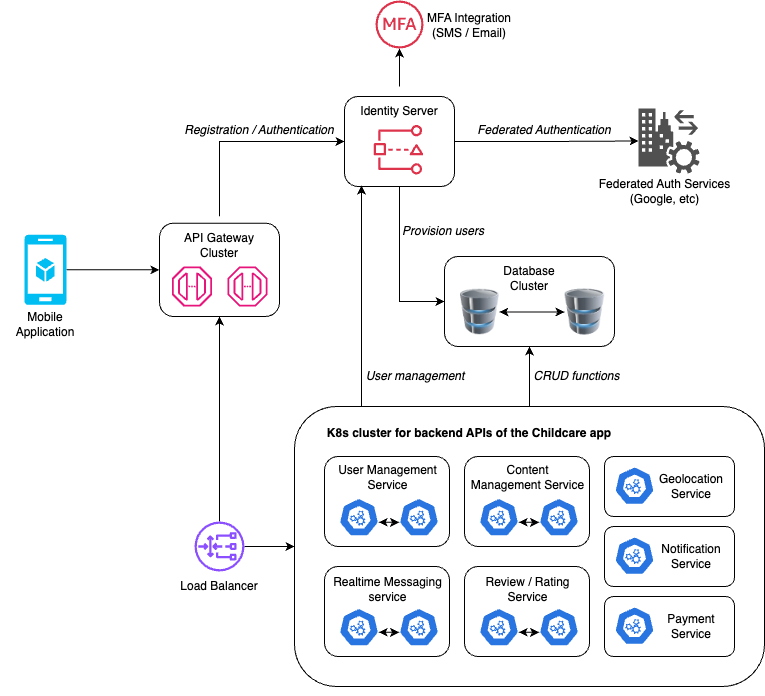
\includegraphics[width=0.55\textwidth,keepaspectratio]{Figures/diagram.png}}}
% 	\caption{Deployment diagram design}%
% 	\label{fig:deploymentdiagram}%
% \end{figure*}

\begin{figure}[htp]
	\center
	{{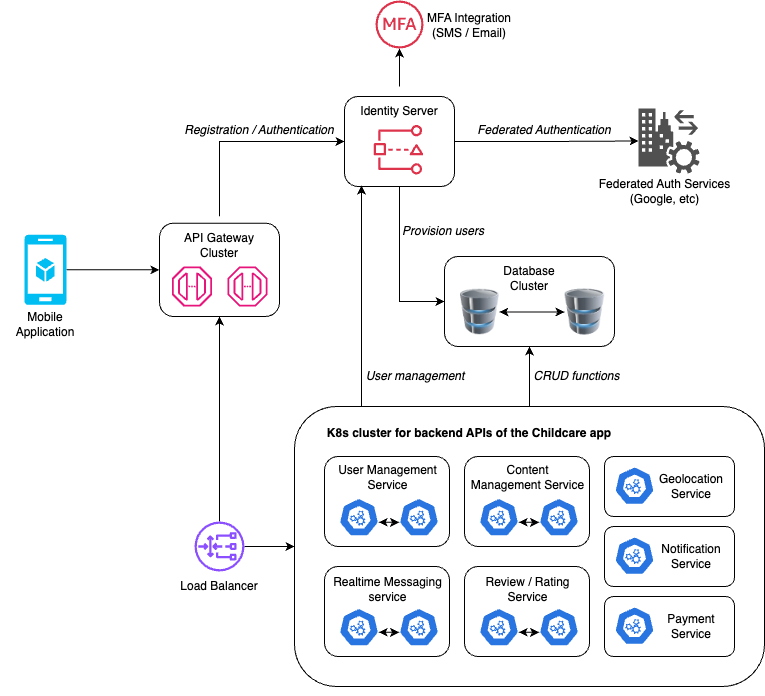
\includegraphics[width=0.9\columnwidth,keepaspectratio]{Figures/diagram.png}}}
	\caption{Deployment design diagram in high-level}%
	\label{fig:deploymentdiagram}%
\end{figure}